\documentclass[11pt]{article}

\usepackage[margin=1in]{geometry}
\usepackage[T1]{fontenc}
\usepackage[utf8]{inputenc}
\usepackage{lmodern}
\usepackage{microtype}
\usepackage{amsmath,amssymb}
\usepackage{booktabs}
\usepackage{array}
\usepackage{tabularx}
\usepackage{multirow}
\usepackage{graphicx}
\usepackage{xcolor}
\usepackage{tikz}
\usepackage{pgfplots}
\usepackage{enumitem}
\usepackage{float}
\usepackage{seqsplit}
\usepackage{hyperref}
\usepackage{bookmark}

\pgfplotsset{compat=1.18}
\usetikzlibrary{arrows.meta,positioning,fit,calc,shapes.geometric}

\definecolor{cacheblue}{HTML}{2D6CDF}
\definecolor{stalered}{HTML}{C3423F}
\definecolor{currentgreen}{HTML}{2E8B57}
\definecolor{lineagepurple}{HTML}{6B4E9B}
\definecolor{neutralgray}{HTML}{5B6470}
\definecolor{lightgray}{HTML}{F2F4F7}

\newcommand{\fullcache}{\texttt{full\_cache}}
\newcommand{\promptdelete}{\texttt{drop\_stale\_prompt}}
\newcommand{\valueedit}{\texttt{value-only}}
\newcommand{\keyedit}{\texttt{key-only}}
\newcommand{\kvedit}{\texttt{K+V}}
\newcommand{\gemma}{Gemma 4 E4B-it}
\newcommand{\gemmamodel}{\texttt{google/gemma-4-E4B-it}}
\newcommand{\qwenmodel}{\texttt{Qwen/Qwen3.5-9B}}
\newcommand{\qwen}{Qwen2.5-7B-Instruct-4bit}
\newcommand{\metrictriple}[3]{#1 / #2 / #3}
\newcommand{\artifactpath}[1]{\path{#1}}
\newcommand{\snapshot}[1]{\texttt{\seqsplit{#1}}}

\title{\textbf{Lineage-Guided Stale-Memory Repair for Reused Transformer KV Caches}\\
\large A Systems Contract for Historical Retention, Operational Freshness, and Provenance}

\author{
Anonymous Authors\\
Artifact path: \texttt{lineagekv}\\
\texttt{paper/stale\_memory\_kv\_cache\_repair.tex}
}

\date{May 21, 2026}

\begin{document}
\maketitle

\begin{abstract}
Long-lived language-model agents increasingly reuse long-context key-value (KV)
caches across turns to avoid expensive prefill. Reuse is efficient, but it also
creates a systems failure mode: a cache can preserve obsolete memory records
after a user's preferences, task state, policy, or tool outcome has changed. We
study \emph{stale-memory cache repair}: suppressing obsolete facts inside a
live transformer KV cache while preserving the full historical memory record.
The method couples a memory-write protocol that records explicit lineage edges
between superseded and current memories with post-prefill cache edits over the
token spans of stale records. A provenance-repair layer then maps generated
evidence aliases back to current memory identifiers. On a 32-case long-context
7B MLX benchmark, value repair matches or improves prompt deletion on answer
and evidence metrics while avoiding full re-prefill, yielding a 15.35x
persistent-update speedup at 6.7k tokens and 38.46x at approximately 32k
tokens. On a raw downloadable \gemma{} checkpoint, a 32-case adversarial
cross-domain matrix shows that full-cache reuse causes wrong or stale actions
in 9/32 cases; prompt deletion prevents 9/9, value-only cache repair prevents
8/9, and key-only or K+V repair prevents 7/9, with no introduced wrong actions.
The results support a practical systems claim rather than a universal
mechanistic law: stale-cache repair is a real intervention class, but the best
edit depends on model family, prompt interface, memory domain, and provenance
requirements. The present evidence base is controlled and intentionally scoped;
decisive journal claims require additional full-precision 7B+ GPU replication,
non-synthetic traces, lineage-noise tests, and stronger cache-management
baselines.
\end{abstract}

\noindent\textbf{Keywords:} transformer inference, KV cache, long-context
agents, memory systems, retrieval, provenance, stale data, model editing,
agent safety.

\section{Introduction}

Transformer inference is increasingly stateful. Production systems cache
prefill activations, reuse context across turns, retrieve external memories,
and ask a model to act on accumulated facts. This architecture makes agents
faster and more useful, but it also creates a subtle mismatch between
\emph{historical memory} and \emph{current operational state}. Historical
records should often remain available for audit, temporal reasoning, and user
trust. Operational decisions, however, should use the current record. If a
system simply reuses a long-context KV cache that contains an obsolete memory,
the model can act on stale content even when the memory store already knows
that a newer record supersedes it.

The conventional fix is prompt deletion: remove obsolete records from the
prompt and rebuild the prefill cache. Prompt deletion is simple and strong, but
it has two drawbacks. First, it destroys the distinction between retaining
history and using history for action. Second, in long contexts it forces a full
prefill refresh after each relevant memory update. This is increasingly costly
as context windows and agent memory stores grow.

This paper studies an alternative: \emph{lineage-guided KV cache repair}. At
memory-write time, the system records which memory records supersede earlier
records. At runtime, the renderer maps memory records to token spans. After
prefill, the inference runtime edits selected key and/or value vectors for
token spans corresponding to stale memories. The full prompt and full cache
remain present, but stale influence is suppressed. A second deterministic
provenance layer resolves evidence identifiers from the memory lineage graph,
so the model need not regenerate exact source IDs from memory.

The central scientific finding is not that a single edit is universally
correct. The evidence points to a \emph{phase diagram}. In Qwen2.5-style runs,
value edits are often the cleanest intervention: values carry obsolete content,
while keys preserve useful address structure. In \gemma{}, value-only, key-only,
and K+V edits can all fix answer-level behavior on some domains, while
provenance leakage remains domain-dependent. Prompt quality also matters:
\gemma{} is clean on easy action-memory cases under its proper turn format, yet
fails under harder adversarial memory conflicts. Thus, the deployable result is
a two-layer contract: maintain memory lineage, choose a model/domain-appropriate
cache policy, and repair provenance from the memory ledger.

\paragraph{Contributions.}
This manuscript makes five contributions:
\begin{enumerate}[leftmargin=1.5em]
  \item We define stale-memory cache repair as a runtime systems problem for
  long-lived language-model agents that reuse long-context KV caches.
  \item We introduce a lineage-guided cache-edit protocol that preserves
  historical memory records while suppressing stale token spans after prefill.
  \item We provide a provenance-repair layer that decouples behavioral repair
  from exact citation generation.
  \item We report a 7B long-context result with up to 38.46x persistent-update
  speedup and no loss in repaired joint answer/source correctness.
  \item We report a raw \gemma{} 32-case cross-domain matrix showing
  wrong-action prevention by prompt deletion and cache repair, and we organize
  the results into a model/domain phase diagram.
\end{enumerate}

\section{Background and Related Work}

\paragraph{Transformer KV caches.}
Autoregressive transformers cache attention keys and values to avoid
recomputing past activations during decoding \cite{vaswani2017attention}. KV
caches are also central to modern serving systems, where cache memory
management strongly affects throughput and latency. PagedAttention and vLLM
focus on efficient allocation and sharing of KV cache blocks for serving
\cite{kwon2023vllm}; KV quantization work such as KIVI and KVQuant focuses on
compressing caches while preserving quality \cite{liu2024kivi,hooper2024kvquant}.
Our work is complementary: we do not primarily compress or page the cache; we
edit semantically stale spans inside it.

\paragraph{KV cache retention, eviction, and streaming.}
H$_2$O, Scissorhands, and StreamingLLM are the closest cache-management
neighbors \cite{zhang2023h2o,liu2023scissorhands,xiao2023streamingllm}. H$_2$O
keeps recent and heavy-hitter tokens, Scissorhands retains tokens predicted to
remain important, and StreamingLLM preserves attention-sink tokens with a
sliding window for stable streaming. These systems decide which KV entries to
retain under memory or sequence-length constraints. Stale-memory repair has a
different objective: a low-rank or low-salience token may still be current, and
a high-attention token may be obsolete. The selection signal is memory lineage,
not attention magnitude or recency. This distinction motivates direct
comparisons to eviction and attention-mask baselines in future revisions.

\paragraph{Prompt and prefix caching.}
Prompt Cache and vLLM automatic prefix caching reuse previously computed
attention states for shared prompt prefixes \cite{gim2024promptcache,kwon2023vllm}.
Commercial prompt-caching APIs expose related serving semantics: users receive
latency or cost benefits when long prompt prefixes are reused, while cache
validity is generally tied to exact or near-exact prefix reuse rather than
semantic freshness. Our setting asks what a serving system should do when the
cached prefix is computationally reusable but operationally stale.

\paragraph{Long-context and memory-augmented language models.}
Retrieval-augmented generation and retrieval-enhanced transformers condition
language models on external text rather than relying solely on parametric
memory \cite{lewis2020rag,borgeaud2022retro}. Long-context transformers and
segment recurrence methods extend the range of usable context
\cite{dai2019transformerxl}. Agent systems add persistent memories that can be
queried across sessions; examples include OS-inspired memory orchestration in
MemGPT/Letta \cite{packer2023memgpt}. These systems generally focus on what to
retrieve, store, summarize, or page. We focus on what happens when retrieved or
cached memory is obsolete but still historically valid.

\paragraph{Model editing and activation intervention.}
Model editing methods modify parameters or internal activations to change model
facts. Stale-memory cache repair is narrower and more operational: the memory
store already knows which record is current, and the objective is not to
rewrite model weights but to repair a live cache state created by a particular
prompt. This makes the intervention reversible, source-local, and compatible
with normal inference.

\paragraph{Provenance and source attribution.}
Citation correctness is a separate requirement from answer correctness. In
agentic systems, a stale action can occur even when the answer text looks
plausible; conversely, a model can answer correctly while citing stale memory.
We therefore measure answer accuracy, evidence accuracy, stale-use rate,
action success, and repaired joint correctness. This separation is important
throughout the results.

\section{Problem Setting}

Let a memory store contain records
\[
  m_i = (\mathrm{id}_i, k_i, x_i, t_i, s_i, \mu_i),
\]
where $\mathrm{id}_i$ is a source identifier, $k_i$ is a memory key, $x_i$ is
text, $t_i$ is a timestamp, $s_i$ is a status, and $\mu_i$ is metadata. A newer
record $m_j$ may supersede an older record $m_i$. We represent this by a
directed lineage edge
\[
  m_i \rightarrow m_j,
\]
meaning that $m_i$ is historically retained but should not control current
actions for the superseded key.

For a rendered prompt prefix $P$, let $T_i \subset \{1,\ldots,|P|\}$ be the
token positions corresponding to memory record $m_i$. A prefill pass produces a
per-layer KV cache
\[
  C = \{(K_\ell, V_\ell)\}_{\ell=1}^{L}.
\]
The stale-memory repair task is to construct a repaired cache $C'$ such that:
\begin{enumerate}[leftmargin=1.5em]
  \item obsolete records remain present in the historical prompt and audit log,
  \item stale token spans exert less influence on current answers and actions,
  \item current records remain available for evidence and reasoning, and
  \item the update path avoids full prompt re-prefill when possible.
\end{enumerate}

\paragraph{Policies.}
We compare:
\begin{itemize}[leftmargin=1.5em]
  \item \fullcache: prefill and decode from the full prompt containing current,
  stale, and distractor memories.
  \item \promptdelete: remove stale records from the prompt before prefill.
  \item \valueedit: keep the full cache but edit selected stale value vectors.
  \item \keyedit: keep the full cache but edit selected stale key vectors.
  \item \kvedit: edit both stale key and stale value vectors.
\end{itemize}

Three natural baselines are not yet in the reported matrix and should be
treated as required revisions before a strong journal claim: attention masking
over stale prefix positions at decode time, span eviction with positional
renumbering, and a current-only retrieval/RAG baseline that rebuilds the prompt
from current memories only. We list them explicitly because they are closer
competitors than \promptdelete{} for some serving deployments, and the present
manuscript should not be read as having ruled them out.

The concrete cache-editing policies used in the raw \gemma{} matrix edit
lineage-conflict spans over layers 8--23. The 7B MLX long-context run uses a
value policy over the same middle-layer band. This band was selected on
development slices; a complete layer sweep is a required next validation. Some
development scripts support current-span scaling, but the reported main rows
use factor 1.0, so this manuscript does not claim a current-boost benefit.

\section{Method}

\subsection{Memory Lineage Protocol}

The memory protocol records supersession at write time. When a new memory is
written to the same operational key, the old current memory is not deleted. It
is marked superseded, and a lineage edge from old to new is stored. The
renderer can then emit a full history prompt with neutral block aliases while
retaining a private map from aliases to memory IDs.

\begin{figure}[H]
\centering
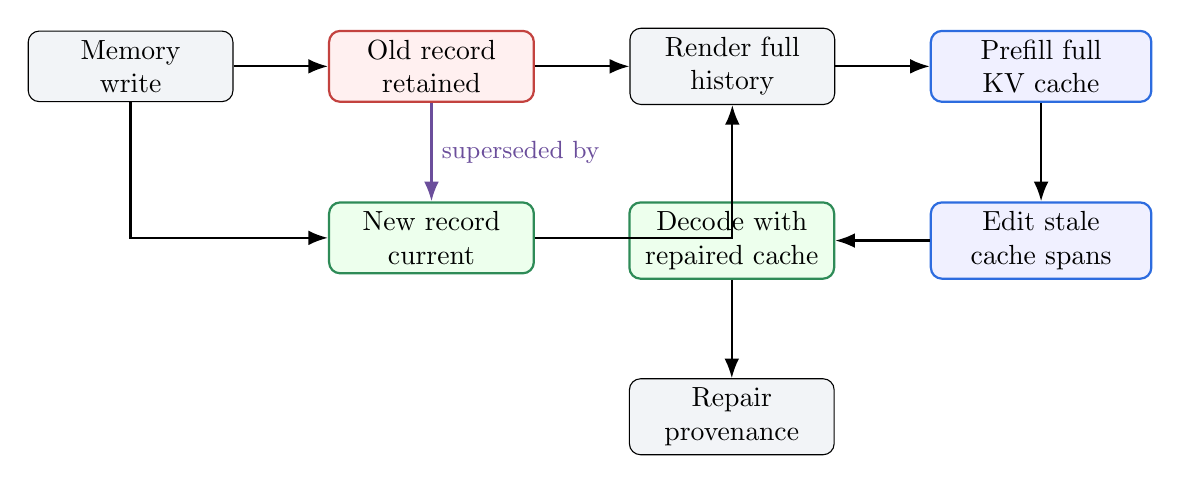
\begin{tikzpicture}[
  node distance=1.25cm and 1.2cm,
  block/.style={draw, rounded corners, align=center, minimum width=2.6cm, minimum height=0.85cm, fill=lightgray},
  stale/.style={draw=stalered, thick, rounded corners, align=center, minimum width=2.6cm, minimum height=0.85cm, fill=red!6},
  current/.style={draw=currentgreen, thick, rounded corners, align=center, minimum width=2.6cm, minimum height=0.85cm, fill=green!7},
  repair/.style={draw=cacheblue, thick, rounded corners, align=center, minimum width=2.8cm, minimum height=0.85cm, fill=blue!6},
  arrow/.style={-{Latex[length=2.5mm]}, thick}
]
\node[block] (write) {Memory\\write};
\node[stale, right=of write] (old) {Old record\\retained};
\node[current, below=of old] (new) {New record\\current};
\node[block, right=of old] (render) {Render full\\history};
\node[repair, right=of render] (prefill) {Prefill full\\KV cache};
\node[repair, below=of prefill] (edit) {Edit stale\\cache spans};
\node[current, left=of edit] (decode) {Decode with\\repaired cache};
\node[block, below=of decode] (prov) {Repair\\provenance};

\draw[arrow] (write) -- (old);
\draw[arrow] (write) |- (new);
\draw[arrow, lineagepurple] (old) -- node[right, font=\small] {superseded by} (new);
\draw[arrow] (old) -- (render);
\draw[arrow] (new) -| (render);
\draw[arrow] (render) -- (prefill);
\draw[arrow] (prefill) -- (edit);
\draw[arrow] (edit) -- (decode);
\draw[arrow] (decode) -- (prov);
\end{tikzpicture}
\caption{Lineage-guided cache repair. Historical records remain in memory and
in the full prompt. Lineage identifies stale spans; cache repair suppresses
their live influence after prefill; provenance repair maps citations back to
current memory IDs.}
\label{fig:method-flow}
\end{figure}

\subsection{Cache Editing}

Let $S$ be the union of stale token spans selected by lineage and rendering:
\[
  S = \bigcup_{m_i \rightarrow m_j} T_i.
\]
Let $\mathcal{L}$ be the selected layer set. A simple value-zeroing policy is:
\[
  V'_{\ell,p} =
  \begin{cases}
    0, & \ell \in \mathcal{L},\ p \in S,\\
    V_{\ell,p}, & \text{otherwise}.
  \end{cases}
\]
Key-only and K+V variants apply the analogous edit to $K_{\ell,p}$ or to both
$K_{\ell,p}$ and $V_{\ell,p}$. The cache edit is local to the current
inference run and does not alter model weights or delete memory records.

\begin{figure}[H]
\centering
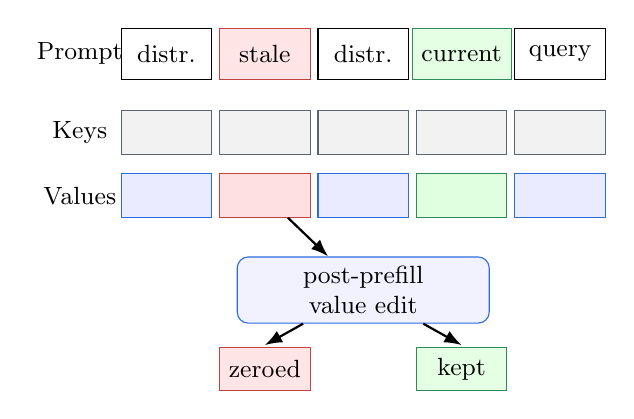
\begin{tikzpicture}[
  every node/.style={font=\small},
  token/.style={draw, minimum width=1.15cm, minimum height=0.65cm},
  stale/.style={draw=stalered, fill=red!10, minimum width=1.15cm, minimum height=0.65cm},
  current/.style={draw=currentgreen, fill=green!10, minimum width=1.15cm, minimum height=0.65cm},
  key/.style={draw=neutralgray, fill=gray!10, minimum width=1.15cm, minimum height=0.55cm},
  val/.style={draw=cacheblue, fill=blue!8, minimum width=1.15cm, minimum height=0.55cm},
  arrow/.style={-{Latex[length=2.2mm]}, thick}
]
\node at (-1.1,0) {Prompt};
\node[token] (d1) at (0,0) {distr.};
\node[stale] (s1) at (1.25,0) {stale};
\node[token] (d2) at (2.5,0) {distr.};
\node[current] (c1) at (3.75,0) {current};
\node[token] (q) at (5.0,0) {query};

\node at (-1.1,-1.0) {Keys};
\foreach \x in {0,1.25,2.5,3.75,5.0} {
  \node[key] at (\x,-1.0) {};
}
\node at (-1.1,-1.8) {Values};
\node[val] at (0,-1.8) {};
\node[val, draw=stalered, fill=red!12] (sv) at (1.25,-1.8) {};
\node[val] at (2.5,-1.8) {};
\node[val, draw=currentgreen, fill=green!12] at (3.75,-1.8) {};
\node[val] at (5.0,-1.8) {};

\node[draw=cacheblue, rounded corners, align=center, fill=blue!5, minimum width=3.2cm] (edit) at (2.5,-3.0) {post-prefill\\value edit};
\draw[arrow] (sv) -- (edit);
\node[stale, minimum width=1.15cm, minimum height=0.55cm] at (1.25,-4.0) {zeroed};
\node[current, minimum width=1.15cm, minimum height=0.55cm] at (3.75,-4.0) {kept};
\draw[arrow] (edit) -- (1.25,-3.7);
\draw[arrow] (edit) -- (3.75,-3.7);
\end{tikzpicture}
\caption{Schematic value-only repair. The full prompt remains present, but
value vectors for lineage-stale token spans are suppressed after prefill. The
production system can choose value-only, key-only, or K+V edits depending on
the measured phase diagram.}
\label{fig:cache-edit}
\end{figure}

\subsection{Provenance Repair}

Generated evidence IDs are fragile because a model may produce a neutral alias,
a stale alias, or a malformed citation even when the answer text is correct.
We therefore distinguish model-generated evidence accuracy from repaired
evidence accuracy. Provenance repair uses the same lineage graph that drives
cache editing:
\[
  \mathrm{repairEvidence}(m_i) =
  \begin{cases}
    m_j, & m_i \rightarrow m_j,\\
    m_i, & \text{otherwise}.
  \end{cases}
\]
This operation does not change the answer text. It provides a deterministic
source contract for downstream systems that need current memory IDs.

\section{Experimental Design}

\subsection{Datasets and Tasks}

Table~\ref{tab:datasets} summarizes the principal datasets and artifacts used
in this manuscript. The benchmarks are generated assistant-memory and
adversarial-lineage tasks plus public Git-history document-revision traces. We
use generated tasks because they provide exact stale/current provenance and
allow paired interventions over identical memory conflicts. This is also a
limitation: the results should be interpreted as controlled systems evidence,
not production telemetry.

\begin{table}[H]
\centering
\small
\begin{tabularx}{\linewidth}{lrrX}
\toprule
\textbf{Dataset / artifact} & \textbf{Cases} & \textbf{Stale IDs} & \textbf{Purpose} \\
\midrule
Public stale-memory benchmark v1 & 184 & 224 & Public assistant-memory benchmark covering nonce updates, action memory, and messy multi-update memory. \\
Universality trace benchmark & 264 & 304 & Mixed benchmark: assistant-memory rows plus public Git-history document-revision rows. \\
MLX long-context action memory & 32 & 32 & 7B long-context quality and persistent-update timing at about 6.7k tokens. \\
Exact-32k runtime slice & 2 & 2 & Long-context externality check at approximately 32k tokens. \\
Raw \gemma{} adversarial lineage & 32 & variable & Cross-domain full/value/key/K+V matrix under proper Gemma turn formatting. \\
\bottomrule
\end{tabularx}
\caption{Datasets and artifacts used in the main evidence package. Stale IDs
refer to records marked stale by lineage or text+timestamp currentness.}
\label{tab:datasets}
\end{table}

\subsection{Models and Runtimes}

The strongest systems result uses \qwen{} in MLX. The raw-model award-track
replication uses \gemma{} through Transformers CPU with bfloat16. The exact
local Hugging Face model ID is \gemmamodel{}, snapshot
\snapshot{d6436b3d62967e1af08bbb046c6300b2a9ae8e85}. We also checked raw
\qwenmodel{} cache compatibility at snapshot
\snapshot{c202236235762e1c871ad0ccb60c8ee5ba337b9a}; it exposes editable KV
tensors only on a subset of hybrid-attention layers, and local CPU decoding is
too slow for benchmark-scale answer-quality runs. Ollama behavioral checks are
excluded from the mechanism claim because they do not expose editable KV
caches.

\subsection{Metrics}

All quality metrics are computed by a deterministic grader over parsed JSON or
the fallback answer string. The grader matches current/stale values and memory
IDs from the benchmark ledger; it does not use an LLM judge. We report:
\begin{itemize}[leftmargin=1.5em]
  \item \textbf{Accuracy}: whether the answer contains the current gold value.
  \item \textbf{Evidence accuracy}: whether generated evidence IDs point to the
  gold current memory.
  \item \textbf{Stale-use rate}: whether the answer or evidence uses a stale
  value, stale evidence ID, or lineage-superseded alias.
  \item \textbf{Wrong-action rate}: one minus action success, where action
  success requires correctness and no stale use.
  \item \textbf{Repaired joint accuracy}: answer correctness together with
  provenance repaired to the current memory ID.
  \item \textbf{Persistent-update speedup}: prompt-deletion update time divided
  by cache-repair update time.
\end{itemize}

\section{Main Results}

\subsection{Raw \gemma{} Cross-Domain Matrix}

Table~\ref{tab:gemma-main} gives the 32-case raw \gemma{} result. Full-cache
reuse fails on both answers and provenance. Prompt deletion is a strong upper
baseline. Cache repair closes the answer gap for all tested edit types, while
value-only repair has the lowest stale-use rate among cache edits.
Because the matrix has only 32 paired cases, one-row differences matter: the
value-only advantage over key-only and K+V is a one-case stale-use margin, not
a settled statistical ordering. A journal revision should add paired bootstrap
intervals or McNemar tests to every cell and comparator.

\begin{table}[H]
\centering
\small
\begin{tabular}{lrrrrr}
\toprule
\textbf{Policy} & \textbf{Cases} & \textbf{Accuracy} & \textbf{Evidence} & \textbf{Stale use} & \textbf{Action success} \\
\midrule
\fullcache & 32 & 0.8125 & 0.6563 & 0.2813 & 0.7188 \\
\promptdelete & 32 & 1.0000 & 1.0000 & 0.0000 & 1.0000 \\
\valueedit & 32 & 1.0000 & 0.9375 & 0.0313 & 0.9688 \\
\keyedit & 32 & 1.0000 & 0.9375 & 0.0625 & 0.9375 \\
\kvedit & 32 & 1.0000 & 0.9375 & 0.0625 & 0.9375 \\
\bottomrule
\end{tabular}
\caption{Raw \gemma{} adversarial-lineage matrix over seven domains. The
metric triple used elsewhere is accuracy / evidence accuracy / stale-use rate.}
\label{tab:gemma-main}
\end{table}

\begin{figure}[H]
\centering
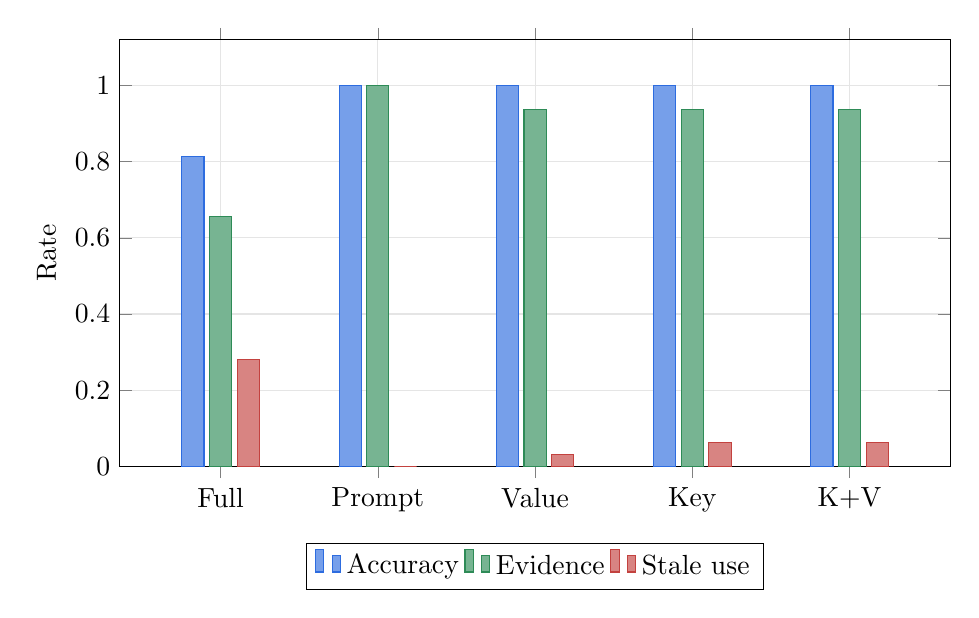
\begin{tikzpicture}
\begin{axis}[
  ybar,
  width=\linewidth,
  height=7cm,
  ymin=0,
  ymax=1.12,
  ylabel={Rate},
  symbolic x coords={Full,Prompt,Value,Key,K+V},
  xtick=data,
  x tick label style={rotate=0, anchor=north},
  bar width=8pt,
  enlarge x limits=0.16,
  legend style={at={(0.5,-0.18)},anchor=north,legend columns=3},
  grid=major,
  major grid style={draw=gray!20}
]
\addplot+[fill=cacheblue!65, draw=cacheblue] coordinates {
  (Full,0.8125) (Prompt,1.0) (Value,1.0) (Key,1.0) (K+V,1.0)
};
\addplot+[fill=currentgreen!65, draw=currentgreen] coordinates {
  (Full,0.65625) (Prompt,1.0) (Value,0.9375) (Key,0.9375) (K+V,0.9375)
};
\addplot+[fill=stalered!65, draw=stalered] coordinates {
  (Full,0.28125) (Prompt,0.0) (Value,0.03125) (Key,0.0625) (K+V,0.0625)
};
\legend{Accuracy,Evidence,Stale use}
\end{axis}
\end{tikzpicture}
\caption{Raw \gemma{} 32-case policy matrix. Cache repair eliminates answer
errors and strongly reduces stale use, but provenance leakage remains policy-
and domain-dependent.}
\label{fig:gemma-bars}
\end{figure}

\subsection{Wrong-Action Prevention}

Table~\ref{tab:wrong-action} shows paired wrong-action prevention relative to
\fullcache. The baseline has nine wrong/stale actions. Prompt deletion prevents
all nine. Value-only cache repair prevents eight, while key-only and K+V
prevent seven. No comparator introduces a new wrong action in this 32-case
matrix.

\begin{table}[H]
\centering
\small
\begin{tabular}{lrrrr}
\toprule
\textbf{Comparator} & \textbf{Baseline wrong} & \textbf{Prevented} & \textbf{Introduced} & \textbf{Prevention rate} \\
\midrule
\promptdelete & 9 & 9 & 0 & 1.000 \\
\valueedit & 9 & 8 & 0 & 0.889 \\
\keyedit & 9 & 7 & 0 & 0.778 \\
\kvedit & 9 & 7 & 0 & 0.778 \\
\bottomrule
\end{tabular}
\caption{Wrong-action prevention on the raw \gemma{} 32-case matrix. A wrong
action is an incorrect or stale-contaminated answer.}
\label{tab:wrong-action}
\end{table}

\begin{figure}[H]
\centering
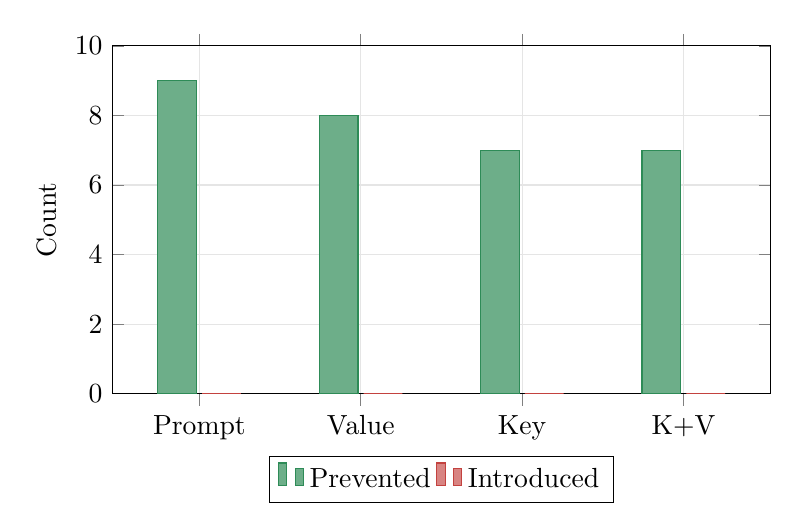
\begin{tikzpicture}
\begin{axis}[
  ybar,
  width=0.82\linewidth,
  height=6cm,
  ymin=0,
  ymax=10,
  ylabel={Count},
  symbolic x coords={Prompt,Value,Key,K+V},
  xtick=data,
  bar width=14pt,
  enlarge x limits=0.18,
  legend style={at={(0.5,-0.18)},anchor=north,legend columns=2},
  grid=major,
  major grid style={draw=gray!20}
]
\addplot+[fill=currentgreen!70, draw=currentgreen] coordinates {
  (Prompt,9) (Value,8) (Key,7) (K+V,7)
};
\addplot+[fill=stalered!65, draw=stalered] coordinates {
  (Prompt,0) (Value,0) (Key,0) (K+V,0)
};
\legend{Prevented,Introduced}
\end{axis}
\end{tikzpicture}
\caption{Paired wrong-action prevention relative to \fullcache{} on raw
\gemma{}.}
\label{fig:wrong-actions}
\end{figure}

\subsection{Domain Phase Diagram}

The domain breakdown in Table~\ref{tab:domain-phase} is the main reason we
avoid a universal-law claim. Some domains show answer/action failures; others
show only provenance failures; one knowledge-base block is clean under proper
prompting. The method is therefore best understood as a policy surface over
model family, interface, domain, and provenance requirement.
The positive stale-use signal is concentrated in five of the seven rows:
deployment-state and knowledge-base have zero full-cache stale-use in this
matrix and should be read as citation-precision or negative-boundary checks,
not evidence for stale-action repair.

\begin{table}[H]
\centering
\scriptsize
\begin{tabularx}{\linewidth}{lrrrrX}
\toprule
\textbf{Domain} & \textbf{Cases} & \textbf{Full acc.} & \textbf{Full ev.} & \textbf{Full stale} & \textbf{Interpretation} \\
\midrule
User preference & 8 & 0.625 & 0.625 & 0.375 & Stale user preference causes wrong actions; all cache edits are clean. \\
Policy approval & 4 & 1.000 & 0.500 & 0.500 & Answer text survives, but stale evidence leaks; value-only is safest before provenance repair. \\
CRM follow-up & 4 & 0.500 & 0.500 & 0.500 & Operational wrong-action domain; all cache edits are clean. \\
Deployment state & 4 & 1.000 & 0.500 & 0.000 & Citation-precision domain; key and K+V repair recover exact evidence. \\
Tool trace & 4 & 1.000 & 0.750 & 0.250 & Stale execution provenance appears despite correct answer. \\
Task state & 4 & 0.750 & 0.750 & 0.250 & Work-tracking stale state; all cache edits are clean. \\
Knowledge base & 4 & 1.000 & 1.000 & 0.000 & Clean under proper Gemma prompt; no repair upside visible. \\
\bottomrule
\end{tabularx}
\caption{Raw \gemma{} domain phase diagram under the proper Gemma turn format.
Columns report \fullcache{} behavior.}
\label{tab:domain-phase}
\end{table}

\begin{figure}[H]
\centering
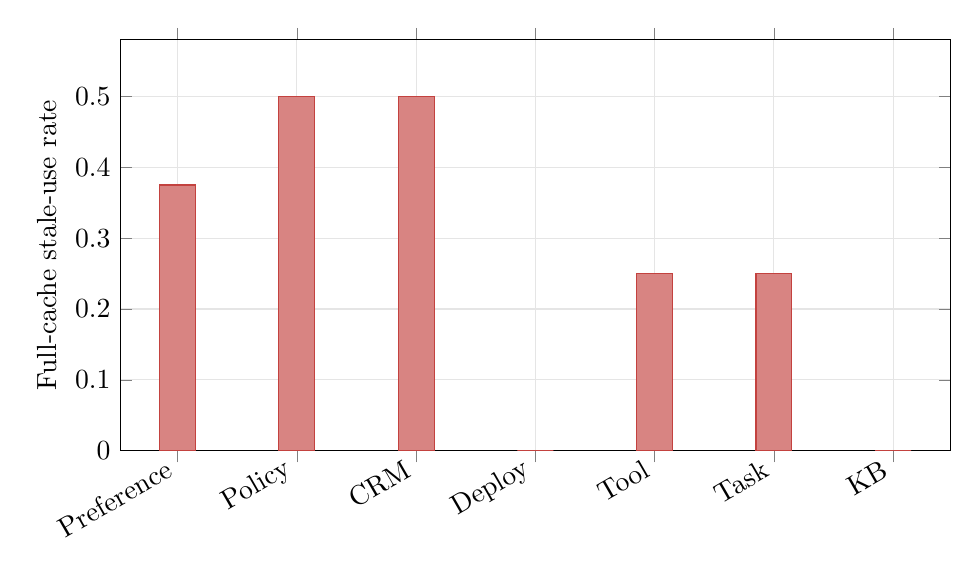
\begin{tikzpicture}
\begin{axis}[
  ybar,
  width=\linewidth,
  height=6.8cm,
  ymin=0,
  ymax=0.58,
  ylabel={Full-cache stale-use rate},
  symbolic x coords={Preference,Policy,CRM,Deploy,Tool,Task,KB},
  xtick=data,
  x tick label style={rotate=30, anchor=east},
  bar width=13pt,
  enlarge x limits=0.08,
  grid=major,
  major grid style={draw=gray!20}
]
\addplot+[fill=stalered!65, draw=stalered] coordinates {
  (Preference,0.375)
  (Policy,0.5)
  (CRM,0.5)
  (Deploy,0.0)
  (Tool,0.25)
  (Task,0.25)
  (KB,0.0)
};
\end{axis}
\end{tikzpicture}
\caption{Full-cache stale-use rate varies by domain. This motivates
model/domain-specific policy selection rather than one universal edit rule.}
\label{fig:domain-stale}
\end{figure}

\subsection{Provenance Repair}

Table~\ref{tab:provenance} shows the effect of deterministic provenance repair
on the raw \gemma{} matrix. Cache edits already recover answer accuracy, but
model-generated evidence remains imperfect. Provenance repair restores all
cache policies to 1.000 repaired joint correctness.

\begin{table}[H]
\centering
\small
\begin{tabular}{lrrrrr}
\toprule
\textbf{Policy} & \textbf{Accuracy} & \textbf{Original ev.} & \textbf{Original joint} & \textbf{Repaired ev.} & \textbf{Repaired joint} \\
\midrule
\promptdelete & 1.0000 & 1.0000 & 1.0000 & 1.0000 & 1.0000 \\
\fullcache & 0.8125 & 0.6563 & 0.6563 & 1.0000 & 0.8125 \\
\valueedit & 1.0000 & 0.9375 & 0.9375 & 1.0000 & 1.0000 \\
\keyedit & 1.0000 & 0.9375 & 0.9375 & 1.0000 & 1.0000 \\
\kvedit & 1.0000 & 0.9375 & 0.9375 & 1.0000 & 1.0000 \\
\bottomrule
\end{tabular}
\caption{Provenance repair on raw \gemma{}. Deterministic lineage repair fixes
source IDs, but it does not rescue wrong answers from \fullcache{}.}
\label{tab:provenance}
\end{table}

\subsection{7B Long-Context Runtime Utility}

The raw \gemma{} result establishes a second-family repair surface, but the
strongest systems utility result comes from the MLX \qwen{} long-context
benchmark. Table~\ref{tab:mlx7b} reports the quality result on 32 held-out
long-context cases.

\begin{table}[H]
\centering
\small
\begin{tabular}{lrrrr}
\toprule
\textbf{Policy} & \textbf{Cases} & \textbf{Accuracy} & \textbf{Evidence} & \textbf{Stale use} \\
\midrule
\fullcache & 32 & 1.0000 & 0.7500 & 0.2500 \\
\promptdelete & 32 & 1.0000 & 0.9375 & 0.0000 \\
Value repair (no boost) & 32 & 1.0000 & 0.9688 & 0.0313 \\
\bottomrule
\end{tabular}
\caption{MLX \qwen{} long-context 32-case result at approximately 6.7k
tokens. With deterministic provenance repair, repaired evidence and repaired
joint correctness reach 1.0000.}
\label{tab:mlx7b}
\end{table}

The paired bootstrap statistics for cache repair versus \fullcache{} on this
7B run show an evidence delta of +0.219 with confidence interval
[0.094, 0.375], and a stale-use delta of -0.219 with confidence interval
[-0.375, -0.094]. Answer accuracy is unchanged at 1.000.

\subsection{Runtime Scaling}

Table~\ref{tab:runtime} and Figure~\ref{fig:runtime} report the persistent
update path. Prompt deletion requires a fresh shorter prefill. Cache repair
reuses the full cache and edits stale spans. The speedup grows with context
length: 15.35x at about 6.7k tokens and 38.46x at about 32k tokens. The ratio
is expected to grow with context because prompt deletion repeats prefill while
the edit path is closer to span-local; the primary measurement is therefore the
absolute update time in milliseconds.

\begin{table}[H]
\centering
\small
\begin{tabular}{lrrrr}
\toprule
\textbf{Context scale} & \textbf{Cases} & \textbf{Prompt deletion} & \textbf{Cache repair} & \textbf{Speedup} \\
 & & \textbf{update ms} & \textbf{update ms} & \\
\midrule
6.7k d48/s4 & 32 & 19,380.0 & 1,262.3 & 15.35x \\
31k d230/s4 & 4 & 85,253.8 & 2,247.4 & 37.93x \\
32k d236/s4 & 2 & 119,077.0 & 3,096.5 & 38.46x \\
\bottomrule
\end{tabular}
\caption{Persistent-update utility for MLX \qwen{}.}
\label{tab:runtime}
\end{table}

\begin{figure}[H]
\centering
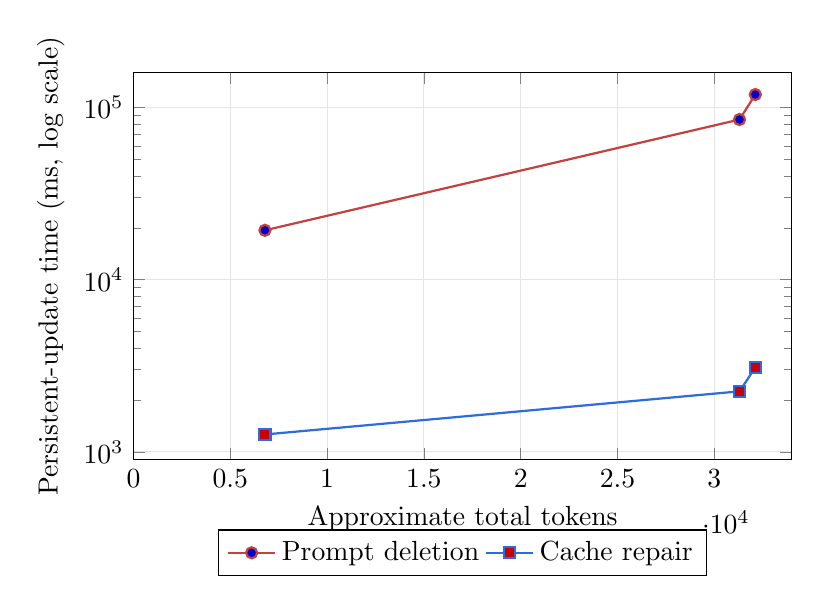
\begin{tikzpicture}
\begin{axis}[
  width=0.82\linewidth,
  height=6.5cm,
  xlabel={Approximate total tokens},
  ylabel={Persistent-update time (ms, log scale)},
  xmin=0,
  xmax=34000,
  ymode=log,
  ymin=900,
  ymax=160000,
  grid=major,
  major grid style={draw=gray!20},
  legend style={at={(0.5,-0.18)},anchor=north,legend columns=2},
  every axis plot/.append style={thick}
]
\addplot+[mark=*, color=stalered] coordinates {
  (6790,19380.0)
  (31300,85253.8)
  (32115,119077.0)
};
\addplot+[mark=square*, color=cacheblue] coordinates {
  (6790,1262.3)
  (31300,2247.4)
  (32115,3096.5)
};
\legend{Prompt deletion,Cache repair}
\end{axis}
\end{tikzpicture}
\caption{Absolute persistent-update time. Cache repair avoids full re-prefill;
the speedup ratios in Table~\ref{tab:runtime} are derived from these paired
measurements.}
\label{fig:runtime}
\end{figure}

\section{Ablations and Boundary Results}

\subsection{Address/Content Dissociation in Qwen2.5}

In smaller Qwen2.5 runs, value-only repair is substantially better than
key-only repair. A representative causal-map result is shown in
Table~\ref{tab:qwen-ablation}. We treat this as an exploratory
address/content hypothesis for this model family, not as a proven mechanism.
The key-only collapse could reflect useful-routing damage, but it could also
reflect more mechanical effects such as attention-norm disruption, rotary
position interactions, or distribution shift from hard zeroing. A stronger
mechanistic section would compare zeroing with mean replacement, norm-matched
noise, and attention-weight redistribution probes.

\begin{table}[H]
\centering
\small
\begin{tabular}{llrrr}
\toprule
\textbf{Model} & \textbf{Edit} & \textbf{Accuracy} & \textbf{Evidence} & \textbf{Stale use} \\
\midrule
Qwen2.5-0.5B & full cache & 0.362 & 0.450 & 0.650 \\
Qwen2.5-0.5B & value-only & 0.412 & 0.650 & 0.375 \\
Qwen2.5-0.5B & key-only & 0.087 & 0.000 & 0.000 \\
Qwen2.5-0.5B & K+V & 0.287 & 0.225 & 0.263 \\
\midrule
Qwen2.5-1.5B & full cache & 0.375 & 0.000 & 1.000 \\
Qwen2.5-1.5B & value-only & 0.425 & 0.950 & 0.425 \\
Qwen2.5-1.5B & key-only & 0.150 & 0.025 & 0.175 \\
Qwen2.5-1.5B & K+V & 0.300 & 0.500 & 0.175 \\
\bottomrule
\end{tabular}
\caption{Representative Qwen2.5 exploratory ablation. Unlike the raw \gemma{}
matrix, Qwen2.5 shows a clearer value-only advantage over key editing, but the
mechanistic interpretation remains provisional.}
\label{tab:qwen-ablation}
\end{table}

\subsection{Prompt Interface Boundary}

The raw \gemma{} experiments reveal a prompt-interface boundary. Under a plain
prompt, a four-case action-memory smoke shows strong stale-cache failures and
malformed outputs. Under a minimal text-only implementation of the Gemma 4 turn
format, the easy action-memory slice becomes clean: \fullcache{},
\promptdelete{}, and K+V repair all reach 1.000 accuracy / 1.000 evidence /
0 stale use over eight current-first and stale-first cases. Harder adversarial
lineage cases are still failure-inducing. This distinction matters for
scientific interpretation: repair results should not be attributed to cache
mechanism when the prompt interface itself is invalid.

\subsection{Preliminary Raw Qwen3.5-9B Smoke}

After the initial compatibility check, we added a no-thinking chat-template
path for \qwenmodel{} and ran a small CPU-only behavioral smoke on a
no-distractor adversarial-lineage user-preference slice. This is not the
full-precision CUDA replication requested in Section~\ref{sec:limitations}:
local MPS fails with an incompatible-dimensions error, and CPU decoding through
the torch fallback is too slow for a 32-case matrix. It is nevertheless useful
boundary evidence because the raw checkpoint now produces parseable answers and
the cache edit changes stale behavior.

\begin{table}[H]
\centering
\small
\begin{tabular}{lrrrr}
\toprule
\textbf{Policy} & \textbf{Cases} & \textbf{Accuracy} & \textbf{Evidence} & \textbf{Stale use} \\
\midrule
\fullcache & 4 & 0.250 & 0.000 & 0.750 \\
\promptdelete & 4 & 1.000 & 0.750 & 0.000 \\
Value repair, layers 8--23 & 4 & 1.000 & 0.750 & 0.000 \\
\bottomrule
\end{tabular}
\caption{Preliminary \qwenmodel{} CPU smoke on a no-distractor adversarial
lineage slice. Prompt deletion and value repair both prevent 3/3 full-cache
wrong actions with no introduced wrong actions. Evidence is 0.750 because one
repeated-current case cites earlier current duplicates rather than the latest
current duplicate; no comparator cites stale evidence.}
\label{tab:qwen35-smoke}
\end{table}

\subsection{Targeting Validity}

The final deployment contract does not require hidden stale labels. The public
184-case benchmark has exact lineage and text+timestamp targeting: 224 true
positive stale records, 0 false positives, and 0 false negatives. The mixed
264-row universality trace benchmark is also exact for both lineage and
text+timestamp detectors across 304 stale records. These audits establish that
the cache edit plan can be generated from programmatic currentness rather than
from model reasoning over stale labels.

\section{Discussion}

\subsection{What Is the Discovery?}

In plain terms, the discovery is that stale memories inside a reused
transformer cache can be repaired without deleting the historical record or
rebuilding the whole prompt. The system needs to know which memory superseded
which older memory. Once it has that lineage, it can target the old record's
token spans in the KV cache and suppress their live effect. The old memory
still exists for audit and temporal context, but it stops controlling current
actions.

\subsection{Why Not Just Replace Memories?}

Replacing or deleting memories is sufficient when history is irrelevant and
contexts are short. Long-lived agents need a stricter contract. They should
remember that a meeting used to be in Room 3B, that a policy used to require
approval, or that a tool call previously failed. Those facts can matter for
explanations, audits, and temporal reasoning. The problem is not historical
retention; it is stale operational influence. Cache repair separates these
concerns.

\subsection{Why a Phase Diagram?}

The results do not justify saying that stale memory always lives in values or
that a fixed layer band is universal. Qwen2.5 shows a strong value/content
dissociation. Raw \gemma{} shows that value-only, key-only, and K+V edits can
all fix answers in some domains, while evidence leakage differs by domain.
The right practical abstraction is a phase diagram: choose a repair policy
after measuring the model/runtime/domain regime.

\subsection{Real-World Impact}

The immediate utility is for agents with persistent memory and expensive
long-context prefill. Examples include coding agents, support copilots, CRM
assistants, research assistants, and workflow agents that maintain user or task
state. Consider a support copilot with a cached account history: an old memory
says a customer is approved for an immediate refund, while a later policy
record says refunds over a threshold require fraud-review approval. The old
record should remain auditable because it explains earlier correspondence, but
it should not authorize the current action. Prompt deletion can solve this at
the cost of rebuilding the prefill. Cache repair gives a path to preserve the
full cached history while suppressing obsolete operational influence.

\section{Limitations}
\label{sec:limitations}

\begin{enumerate}[leftmargin=1.5em]
  \item The strongest long-context runtime result uses MLX 4-bit Qwen2.5, not
  full-precision CUDA. A single full-precision 7B+ GPU replication is the
  highest-value next experiment.
  \item The raw \gemma{} matrix is one raw non-Qwen model family on local CPU.
  It is benchmark-scale for this project, but not a broad model zoo.
  \item The principal benchmarks are generated or controlled. They provide
  exact lineage and paired interventions, but they are not production telemetry.
  The public Git-history rows provide a partial non-synthetic anchor, but the
  main 7B and raw-\gemma{} headline tables are generated.
  \item The current main tables lack attention-mask, span-eviction, and
  current-only retrieval baselines. These are required before claiming that KV
  editing is the best available serving strategy.
  \item Statistical reporting is incomplete for the raw \gemma{} matrix. The
  next draft should include paired bootstrap intervals or exact paired tests
  for every main cell and comparator.
  \item The layer band 8--23 is development-selected. We report no layer-band
  sweep or nontrivial $\alpha$ sweep in the main 7B/\gemma{} results; all
  current-boost claims should be withheld until that sweep is run.
  \item The memory ledger integration is demonstrated, but a large deployed
  agent study remains future work.
  \item Provenance repair assumes that the memory store has reliable lineage or
  currentness metadata. We have not yet quantified robustness to missing,
  flipped, or noisy lineage edges. Without reliable lineage, the system should
  fail closed.
  \item Cache edit policies are runtime- and architecture-dependent. Hybrid
  attention models may expose only a subset of editable KV layers.
\end{enumerate}

\section{Ethics and Safety}

Stale-memory repair is a safety mechanism for reducing obsolete instructions
and stale facts in agent decisions. It can also be misused if memory lineage is
incorrectly recorded or if an operator hides historical records while claiming
they are preserved. We therefore recommend auditable memory ledgers, explicit
currentness metadata, conservative fail-closed behavior, and evaluation that
separates answer correctness from provenance correctness. The generated
benchmarks in this work do not contain private user data.

\section{Reproducibility and Artifact Availability}

The repository contains scripts, datasets, result CSVs, and an interactive demo.
Key artifacts include:
\begin{itemize}[leftmargin=1.5em]
  \item \artifactpath{data/public/stale_memory_repair_benchmark_v1.jsonl}
  \item \artifactpath{data/public/stale_memory_universality_traces_v1.jsonl}
  \item \artifactpath{scripts/kv_value_ablation_probe.py}
  \item \artifactpath{scripts/kv_mlx_value_ablation_probe.py}
  \item \artifactpath{src/context_rot/memory/ledger.py}
  \item raw \gemma{} driver: \artifactpath{scripts/kv_value_ablation_probe.py}\\
  \texttt{--model google/gemma-4-E4B-it}\\
  \texttt{--prompt-style gemma4}
  \item \artifactpath{results/kv/kv_gemma4_e4b_adversarial_lineage_crossdomain32_gemma4prompt_matrix_summary.csv}
  \item \artifactpath{results/kv/kv_gemma4_e4b_raw_cache_compat.json}
  \item \artifactpath{results/kv/kv_qwen35_9b_raw_cache_compat.json}
  \item \artifactpath{results/kv/kv_qwen35_9b_adversarial_lineage_d0_probe4_nothink_cpu_summary.csv}
  \item \artifactpath{results/kv/kv_public_runtime_curve.csv}
  \item \artifactpath{demo/kv_memory_repair_demo.html}
\end{itemize}

The no-model public reproduction entry point is:
\begin{verbatim}
bash scripts/run_kv_public_repro.sh
\end{verbatim}

\section{Conclusion}

Reused long-context KV caches create a stale-memory failure mode for long-lived
agents. We show that memory lineage can make stale spans targetable, that
cache edits can suppress stale influence without deleting historical memory,
and that deterministic provenance repair can restore current source IDs. The
strongest systems result shows large update-path speedups at long context. The
raw \gemma{} matrix shows that the repair class transfers beyond the original
Qwen2.5 setting, while also revealing domain and prompt-interface boundaries.
The scientific contribution is therefore a deployable systems contract and a
model/domain phase diagram, not a universal transformer law. The next decisive
step is independent raw 7B+ or full-precision CUDA replication and evaluation
on realistic production-like memory logs.

\appendix

\section{Algorithmic Summary}

\begin{table}[H]
\centering
\small
\begin{tabularx}{\linewidth}{rX}
\toprule
\textbf{Step} & \textbf{Operation} \\
\midrule
1 & Write memory record with key, timestamp, text, status, and source ID. \\
2 & If the key has an earlier current record, mark it superseded and add a lineage edge from old to new. \\
3 & Render full memory history with neutral aliases and record token spans for every memory record. \\
4 & Prefill the model on the full rendered prompt. \\
5 & Build stale token span set from lineage edges and render spans. \\
6 & Apply selected cache edit over selected layers: value-only, key-only, or K+V. \\
7 & Decode from the repaired cache. \\
8 & Repair or verify evidence IDs using the lineage graph before downstream action. \\
\bottomrule
\end{tabularx}
\caption{Lineage-guided stale-memory cache repair algorithm.}
\label{tab:algorithm}
\end{table}

\section{Raw \gemma{} Artifact Map}

\begin{table}[H]
\centering
\scriptsize
\begin{tabularx}{\linewidth}{lX}
\toprule
\textbf{Result} & \textbf{Artifact path} \\
\midrule
32-case matrix summary & \artifactpath{results/kv/kv_gemma4_e4b_adversarial_lineage_crossdomain32_gemma4prompt_matrix_summary.csv} \\
32-case wrong-action summary & \artifactpath{results/kv/kv_gemma4_e4b_adversarial_lineage_crossdomain32_gemma4prompt_matrix_wrong_action_summary.csv} \\
32-case provenance repair summary & \artifactpath{results/kv/kv_gemma4_e4b_adversarial_lineage_crossdomain32_gemma4prompt_matrix_provenance_repair_summary.csv} \\
Raw \gemma{} cache compatibility & \artifactpath{results/kv/kv_gemma4_e4b_raw_cache_compat.json} \\
Raw \qwenmodel{} cache compatibility & \artifactpath{results/kv/kv_qwen35_9b_raw_cache_compat.json} \\
Task-state rows & \artifactpath{results/kv/kv_gemma4_e4b_adversarial_lineage_task_state_offset100_4_gemma4prompt_matrix_cpu.jsonl} \\
Knowledge-base rows & \artifactpath{results/kv/kv_gemma4_e4b_adversarial_lineage_knowledge_base_offset120_4_gemma4prompt_matrix_cpu.jsonl} \\
\bottomrule
\end{tabularx}
\caption{Raw \gemma{} artifacts created for the 32-case matrix.}
\label{tab:artifact-map}
\end{table}

\begin{thebibliography}{99}

\bibitem{vaswani2017attention}
Ashish Vaswani, Noam Shazeer, Niki Parmar, Jakob Uszkoreit, Llion Jones,
Aidan N. Gomez, Lukasz Kaiser, and Illia Polosukhin.
\newblock Attention is all you need.
\newblock In \emph{Advances in Neural Information Processing Systems}, 2017.
\newblock arXiv:1706.03762.

\bibitem{dai2019transformerxl}
Zihang Dai, Zhilin Yang, Yiming Yang, Jaime Carbonell, Quoc V. Le, and
Ruslan Salakhutdinov.
\newblock Transformer-XL: Attentive language models beyond a fixed-length
context.
\newblock In \emph{Proceedings of ACL}, 2019.

\bibitem{lewis2020rag}
Patrick Lewis, Ethan Perez, Aleksandra Piktus, Fabio Petroni, Vladimir
Karpukhin, Naman Goyal, Heinrich Kuttler, Mike Lewis, Wen-tau Yih, Tim
Rocktaschel, Sebastian Riedel, and Douwe Kiela.
\newblock Retrieval-augmented generation for knowledge-intensive NLP tasks.
\newblock In \emph{Advances in Neural Information Processing Systems}, 2020.

\bibitem{borgeaud2022retro}
Sebastian Borgeaud, Arthur Mensch, Jordan Hoffmann, Trevor Cai, Eliza
Rutherford, Katie Millican, George van den Driessche, Jean-Baptiste Lespiau,
Bogdan Damoc, Aidan Clark, Diego de Las Casas, Aurelia Guy, Jacob Menick,
Roman Ring, Tom Hennigan, Saffron Huang, Loren Maggiore, Chris Jones, Albin
Cassirer, Andy Brock, Michela Paganini, Geoffrey Irving, Oriol Vinyals, Simon
Osindero, Karen Simonyan, Jack W. Rae, Erich Elsen, and Laurent Sifre.
\newblock Improving language models by retrieving from trillions of tokens.
\newblock In \emph{Proceedings of ICML}, 2022.
\newblock arXiv:2112.04426.

\bibitem{kwon2023vllm}
Woosuk Kwon, Zhuohan Li, Siyuan Zhuang, Ying Sheng, Lianmin Zheng, Cody Hao
Yu, Joseph E. Gonzalez, Hao Zhang, and Ion Stoica.
\newblock Efficient memory management for large language model serving with
PagedAttention.
\newblock In \emph{Proceedings of SOSP}, 2023.

\bibitem{gim2024promptcache}
In Gim, Guojun Chen, Seung-seob Lee, Nikhil Sarda, Anurag Khandelwal, and
Lin Zhong.
\newblock Prompt Cache: Modular attention reuse for low-latency inference.
\newblock In \emph{Proceedings of MLSys}, 2024.
\newblock arXiv:2311.04934.

\bibitem{zhang2023h2o}
Zhenyu Zhang, Ying Sheng, Tianyi Zhou, Tianlong Chen, Lianmin Zheng, Ruisi Cai,
Zhao Song, Yuandong Tian, Christopher R\'e, Clark Barrett, Zhangyang Wang, and
Beidi Chen.
\newblock H$_2$O: Heavy-hitter oracle for efficient generative inference of
large language models.
\newblock In \emph{Advances in Neural Information Processing Systems}, 2023.
\newblock arXiv:2306.14048.

\bibitem{liu2023scissorhands}
Zichang Liu, Aditya Desai, Fangshuo Liao, Weitao Wang, Victor Xie, Zhaozhuo
Xu, Anastasios Kyrillidis, and Anshumali Shrivastava.
\newblock Scissorhands: Exploiting the persistence of importance hypothesis
for LLM KV cache compression at test time.
\newblock In \emph{Advances in Neural Information Processing Systems}, 2023.
\newblock arXiv:2305.17118.

\bibitem{xiao2023streamingllm}
Guangxuan Xiao, Yuandong Tian, Beidi Chen, Song Han, and Mike Lewis.
\newblock Efficient streaming language models with attention sinks.
\newblock arXiv:2309.17453, 2023.

\bibitem{liu2024kivi}
Zirui Liu, Jiayi Yuan, Hongye Jin, Shaochen Zhong, Zhaozhuo Xu, Vladimir
Braverman, Beidi Chen, and Xia Hu.
\newblock KIVI: A tuning-free asymmetric 2bit quantization for KV cache.
\newblock In \emph{Proceedings of ICML}, 2024.
\newblock arXiv:2402.02750.

\bibitem{hooper2024kvquant}
Coleman Hooper, Sehoon Kim, Hiva Mohammadzadeh, Michael W. Mahoney, Yakun Sophia
Shao, Kurt Keutzer, and Amir Gholami.
\newblock KVQuant: Towards 10 million context length LLM inference with KV
cache quantization.
\newblock arXiv:2401.18079, 2024.

\bibitem{yao2023react}
Shunyu Yao, Jeffrey Zhao, Dian Yu, Nan Du, Izhak Shafran, Karthik Narasimhan,
and Yuan Cao.
\newblock ReAct: Synergizing reasoning and acting in language models.
\newblock In \emph{International Conference on Learning Representations}, 2023.

\bibitem{packer2023memgpt}
Charles Packer, Vivian Fang, Shishir G. Patil, Kevin Lin, Sarah Wooders, and
Joseph E. Gonzalez.
\newblock MemGPT: Towards LLMs as operating systems.
\newblock arXiv:2310.08560, 2023.

\end{thebibliography}

\end{document}
